%# -*- coding: utf-8-unix -*-
\chapter{符号化电路简化原理应用}
\label{chap:application}

本章对之前提出的基于GPDD的电路简化原理以及模拟电路的模型降阶方法给出了相应的应用,并对其具体性能进行了测试分析。

\section{应用一:时域符号化简化模型自动生成方法}

通过上一章的分析,可以看到电路简化模型在频率响应分析上表现出了不错的稳定性与有效性。
本章通过借用前一章分析得到的简化电路模型,尝试构造相应的电路结构,从而得到可以用于时域大信号的电路模型,并通过电路测试结果来显示方法的效果。

\subsection{传统的时域模型分析方法}

对于传统的运算放大器,其阶跃响应输出往往呈现如图\ref{fig:slewmeaning}所表现的形式。

\begin{figure}[!htp]
	\centering
	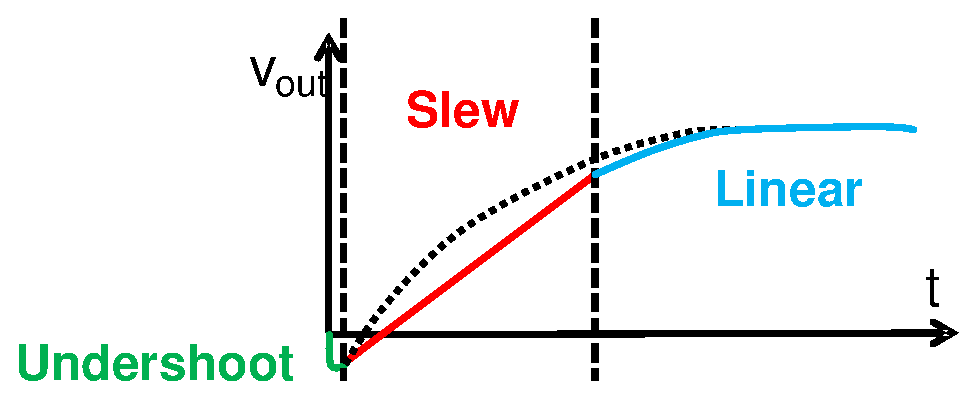
\includegraphics[width=0.6\textwidth]{chap3/SlewMeaning.eps}
	\bicaption[fig:slewmeaning]{Slew-Settling过程}{Slew-Settling过程}{Fig}{Slew-Settling procedure}
\end{figure}

图中,首先绿色部分为Undershoot部分,为线性响应,往往由于运放反馈连接中的零点造成,蓝色部分为Settling过程的线性响应部分。
其中最为关键的是红色的Slew部分。
由于在实际情况中,运放的输出能力有限,不可能输出无限大的电流,所以在运放输出端给输出端所寄生的电容充电的过程中,电压不一定能以线性的工作方式与时间呈指数上升(如黑色虚线所示)。
这种情况下由于电流输出已饱和,基本为以恒定值,故运放输出端电压随时间成比例增长,这条曲线的斜率称之为压摆率(Slew Rate,SR),一般压摆率的估计值可由输出电流$I$与输出端电容$C$的比值决定,如下式所示。

\begin{equation}
	SR = \frac{I}{C}
\end{equation}

为了对运放的Slew-Settling过程进行分析,往往需要对运放的这一过程进行建模。
但是由于上述的公式十分粗糙,很难以用于比较精细的电路分析中。
故有大量研究使用各种方法对运放的时域模型进行建模。
\parencite{Pug-3Segment-2010}提出了三段式模型对这一过程进行建模。所谓三段式模型即根据运放响应的三个不同的过程(Undershoot,Slew,Settling)进行分段处理,从而形成一个用于表示运放行为的分段函数作为模型。
\parencite{Yavari-TSSlew-2005,Rezaee-FCSlew-2009}中使用了大信号分析,从电路器件模型出发,通过直接求解电路微分方程等方法对Slew-Settling行为进行分析。
这两种方式虽然有一定处理此类问题的能力,但是相对来说,其公式处理十分繁琐同时由于电路被抽象成一个个分段函数,同时往往需要计算积分等复杂运算,很难回溯会具体的电路器件进行分析,也很难自动化进行。

1982年,Chuang等人提出了在线性系统中加入限制的方式来模拟电路的Slew-Settling模型\parencite{Chuang-Slew-1982}。
这种方法因其本质上是线性系统,仅通过电流的输出能力大小来限制其输出信号,故比较适用与可以分析零极点的符号化方法。
今年来,G. Shi等人通过结合符号化零极点分析与Chuang的电路模型\parencite{ZhangHe-Slew-2011,ZhangAilin-Slew-2015},提出了使用运放宏模型的方式对运放进行建模。
这种方式不仅更为准确,同时提供了更明确的电路意义。一个二级运算放大器的电路宏模型如下图\ref{fig:macromodel}所示:

\begin{figure}[!htp]
	\centering
	\includegraphics[width=0.6\textwidth]{chap3/macromodel.png}
	\bicaption[fig:macromodel]{运放时域宏模型}{运放时域宏模型\parencite{ZhangAilin-Slew-2015}}{Fig}{Opamp macromodel in time domain\parencite{ZhangAilin-Slew-2015}}
\end{figure}

可以看到通过提取二级运算放大器中各级的零极点,就可以得到每一级中跨导和相应的阻抗与电容。同时注意第一级运放的跨导有电流输出的限制,以模拟运放电路本身的电流输出限制。
那么现在问题就主要在于宏模型电路中各个元件的参数选取上,通过GPDD结构与模比配(Moment Matching)的方法可以得到主要的几阶项,从而得到各级的零极点关系。例如,通过GPDD计算,我们可以得到如下公式:

\begin{equation}
	H\left( s \right) = \frac{{N\left( s \right)}}
	{{D\left( s \right)}} = \frac{{{b_0}{s^0} + {b_1}{s^1} +  \cdots  + {b_q}{s^q}}}
	{{{a_0}{s^0} + {a_1}{s^1} +  \cdots  + {a_r}{s^r}}}
\end{equation}

对上式进行泰勒展开后,可以得到:

\begin{equation}
	{H_{ex}}\left( s \right) = {m_0}{s^0} + {m_1}{s^1} + {m_2}{s^2} +  \cdots
\end{equation}

其中系数可以通过联立上述两个公式后,对公式两边多次求导的方式,逐一得到相应的系数,如下式所示。

\begin{align}
	& m_0 = \frac{b_0}{a_0} \nonumber \\
	& m_1 = \frac{{b_1} - {m_0}{a_1}}{a_0} \nonumber \\
	& m_2 = \frac{{b_2} - {m_0}{a_2} - {m_1}{a_1}}{a_0} 
\end{align}

故宏模型电路中的跨导$G$、电阻$R$和电容$C$可以以上公式计算得到。这样就建立起了宏模型与电路实际元件之间的关系,有利于日后对于电路性能优化的进一步分析。
这种方式的主要优势在于直接将电路模型中的零极点与电路元件关系挂上勾,从而电路模型不仅可以在时域,也可以在频域进行计算。
更主要的是这种模型,传统仿真器中可以简单地通过编写网表得到,仿真方便便捷。

\subsection{符号化时域简化模型分析方法}

\subsubsection{时域符号化简化流程}

本方法的基本流程类似于Chuang模型,首先获取简化的小信号模型,然后在该小信号模型的基础上加入对输出电流饱和的限制。
但是,本方法与Chuang模型有三点不同,分别为:

\begin{enumerate}[label=\emph{\alph*})]
	\item 简化的小信号零极点模型可以直接通过第二章的符号化模型降阶算法得到。
	\item 限制电流加载运放中所有得以保留的$g_m$元件上,并用大信号中的通过管子的电流作为其限制电流。
	\item 采用了更加光滑的非线性函数,以更加真实地模拟实际情况。
\end{enumerate}

\begin{figure}[!htp]
	\centering
	\includegraphics[width=0.6\textwidth]{chap3/CurrentLimitPos.eps}
	\bicaption[fig:limitcur]{时域模型中的电流限制位置}{时域模型中的电流限制位置}{Fig}{Current limit position in slew-settling model}
\end{figure}

其中第一点正是相比之前的方法的闪光点。因为之前的方法,即使是一般的零极点模型,往往很难建立模型与电路元件之间的关系,而给出简化小信号模型可以直观地给出两者之间的联系。

第二点可参考图\ref{fig:limitcur}的示意,本方法将运放电路中所有存在的$g_m$均加入限制。
\parencite{Yavari-TSSlew-2005}中指出,现代的模拟集成电路由于其功耗降低,电源电压降低等原因,造成电流输出饱和的原因不一定是由输入级决定的,可能是之后的电路充电速度不足导致。
Chuang模型中只考虑了第一级电路的输出饱和,对之后级的输出限制没有做出过多考量。
如果在各个$g_m$上加入相应的电流限制,那么即可模拟各级中的电流限制。

\begin{figure}[!htp]
	\centering
	\includegraphics[width=0.8\textwidth]{chap3/gmvariation.eps}
	\bicaption[fig:gmvariation]{Slew-settling过程中输入管$g_m$的变化}{Slew-settling过程中输入管$g_m$的变化}{Fig}{$g_m$ variation during the slew-settling procedure}
\end{figure}

图\ref{fig:gmvariation}给出了两级运算放大器slew-settling的过程中输入管的$g_m$随着输入交流小信号的变化。
图中箭头方向代表了时间的流向。在Slew过程(红色圆圈)中,$g_m$快速爬升至所需要的稳态情况的值;而在Settling过程(蓝色方块)中,$g_m$稳定在某一值不再变化。
以往,我们往往假设$g_m$的函数是一个分段函数,在未饱和前,输入电压和输出电流成正比;饱和后,输出稳定电流。
这样的话$g_m$仅有两个值,其一是稳态情况下的跨导,另一个是$0$。
然而在图中明显看到这样的假设是不合理的,一个办法就是重新决定施加给$g_m$的非线性函数。

\subsubsection{非线性函数选取}

非线性函数有许多不同的形式。
一类合适的函数是S型函数族$S_i\left(x\right)$。
这里列举了五种不同的函数方程共参考:
\begin{align}
	&{S_0}\left( x \right) = \left\{ {\begin{array}{*{20}{c}}1 & {x \geqslant 1}  \\x & { - 1 \leqslant x < 1}  \\{ - 1} & {x < 1}  \\\end{array} } \right. \\
	&{S_1}\left( x \right) = \tanh \left( x \right) \hfill \\
	&{S_2}\left( x \right) = \frac{2}{\pi }gd\left( {\frac{\pi }	{2}x} \right) = \frac{2}{\pi }\arcsin \left( {\tanh \left( {\frac{\pi }{2}x} \right)} \right)\\
	&{S_3}\left( x \right) = \frac{x}{{\sqrt {1 + {x^2}} }}\\
	&{S_4}\left( x \right) = \frac{2}{\pi }\arctan \left( {\frac{\pi }{2}x} \right)
\end{align}

\begin{figure}[!htp]
	\centering
	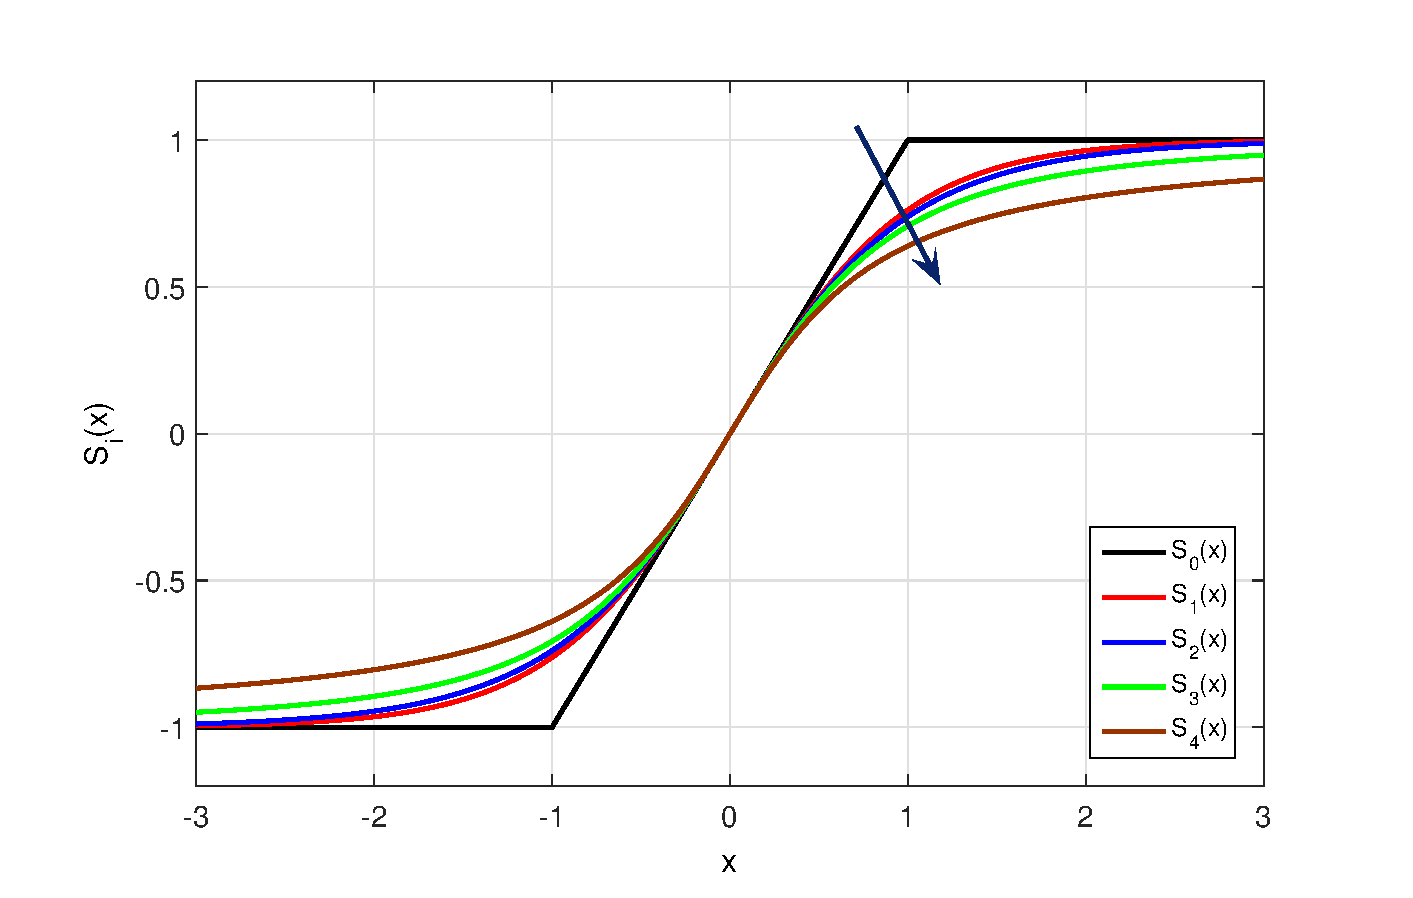
\includegraphics[width=0.8\textwidth]{chap3/sigmoid.eps}
	\bicaption[fig:sigmoid]{S型函数族}{S型函数族}{Fig}{Sigmoid function family}
\end{figure}

图\ref{fig:sigmoid}中展示了所有这5中S型函数的曲线。
可以看到原先在Chuang模型中使用的非线性函数即为这里的$S_0\left(x\right)$。
图中的箭头显示了这些函数在正半平面或负平面中不互相相较,且呈现出了一定顺序。
这类函数有一些共同的特征,如它们都绝对单调递增,可总结如下:

\begin{eqnarray}
	\mathop {\lim }\limits_{x \to  + \infty } {S_i}\left( x \right) = 1\\
	\mathop {\lim }\limits_{x \to  - \infty } {S_i}\left( x \right) = -1\\
	{\left. {\frac{d}{{dx}}{S_i}\left( x \right)} \right|_{x = 0}} = 1
\end{eqnarray}

如果有一个跨导的DC偏置电流是$I_0$,其增益为$g_m$,那么对这类函数只需要做如下的变换即可得到我们所需要的非线性的$g_m$。

\begin{equation}
	{I_0}{S_i}\left( {\frac{{{g_m}}}{{{I_0}}}x} \right)
\end{equation}

\subsection{符号化时域简化模型测试结果}

\subsubsection{两级运放测试结果}

\begin{figure}[!htp]
	\centering
	\includegraphics[width=0.8\textwidth]{chap3/TS_Slew.eps}
	\bicaption[fig:tsslew]{两级运放模型的Slew-Settling时域仿真结果}{两级运放模型的Slew-Settling时域仿真结果}{Fig}{Simulation Results of slew-settling behavior for two-stage opamp model}
\end{figure}

首先我们针对两级运放电路进行了电路时域模型的建模,图\ref{fig:tsslew}中展示了在不同S型函数作用下的电路的Slew-Settling行为。
可以看到$S_0\left(x\right)$、$S_1\left(x\right)$和$S_2\left(x\right)$在Slew阶段表现出了良好的对压摆率的估计行为。
而$S_4\left(x\right)$则非常适于对于电路稳定时间的估计。
这里并没有画出相应的$S_3\left(x\right)$的曲线,因为其HSPICE仿真并不收敛。
可以发现图中的箭头标志了这些函数作用下的时域曲线也呈现了一定的顺序,且与上一小节中的次序一致。
故可以预估$S_3\left(x\right)$会取得最好的电路近似程度。

\subsubsection{折叠共源共栅运放测试结果}

在对折叠共源共栅运放的电路测试中,我们发现只有$S_1\left(x\right)$的作用下,电路才可以顺利由HSPICE求解出来,仿真结果如图\ref{fig:fcslew}。
这里结果十分值得怀疑,因为其中出现了奇怪的折角,这在电路稳定的情况下不应该出现。
同时,此时本方法生成的时域运放模型并不能很好地抓取电路的时域特性,说明时域模型生成方法仍存在一些问题,需要进一步分析验证。

\begin{figure}[!htp]
	\centering
	\includegraphics[width=0.8\textwidth]{chap3/FC_Slew.eps}
	\bicaption[fig:fcslew]{折叠共源共栅运放模型的Slew-Settling时域仿真结果}{折叠共源共栅运放模型的Slew-Settling时域仿真结果}{Fig}{Simulation Results of slew-settling behavior for folded-cascode opamp model}
\end{figure}

\section{应用二:共模电源抑制比符号化分析}

\subsection{共模抑制比与电源抑制比介绍}

运算放大器除了差分增益响应以及相对应的相位变化,别的设计指标也是极为关键的。
在近几年兴起的生物电路中,由于生物电信号的较为微弱的特性,共模及电源噪声信号的影响对相关的运算放大器设计工作提出了很高的要求\parencite{Sawan-CMRR-1999,Abdullah-Biopotential-2015,Paul-22dBPSRR-2012}。
目前对这两方面指标的自动化辅助工具的研究比较欠缺,故十分需要有相应的工具对此种类型的电路分析工作进行指导与辅助。

根据\parencite{GRAY-Analog}中的定义,可根据图\ref{fig:cmps}中的示意给出共模抑制比(Common Mode Rejection Ratio, $CMRR$)和电源抑制比(Power Supply Rejection Ratio, $PSRR$)的定义。

\begin{figure}[!htp]
	\centering
	\includegraphics[width=0.8\textwidth]{chap4/CMPS.eps}
	\bicaption[fig:cmps]{共模抑制比及电源抑制比定义}{共模抑制比及电源抑制比定义}{Fig}{CMRR and PSRR definition}
\end{figure}

首先给出CMRR的定义,如图\ref{fig:cmps}左侧所示,一个差分运算放大器有两个差分输入端,如果在两个输入端输入叠加在共模信号上的差分信号。
用$v_d$和$v_{cm}$代表信号的差模和共模部分,那么我们可以得到运放的输出信号的差模部分有$v_{out}^{d} = A_v v_d$;而共模输出信号有$v_{out}^{cm} = A_{cm} v_{cm}$。
这里$A_v$和$A_{cm}$代表了运放的差模和共模增益。那么可以将CMRR定义为差模增益与共模增益的比值,如下式所示。

\begin{equation}
CMRR = \left|\frac{A_v}{A_{cm}}\right|
\end{equation}

接着给出PSRR的定义,如图\ref{fig:cmps}右侧所示,运放的电源电压部分给上一个小信号激励$v_{dd}$。
那么运放输出中由电源处提供的信号可以表示为$v_{out}^{ps} = A_{ps}v_{dd}$,这里$A_{ps}$代表了运放的电源增益。
故可以将PSRR定义为差模增益与电源增益的比值,如下式所示。

\begin{equation}
PSRR = \left|\frac{A_v}{A_{ps}}\right|
\end{equation}

可以看到运放的CMRR和PSRR均是通过小信号计算得到,故可以使用符号化分析得到相应的结果。
同时可以看到在分析CMRR和PSRR的过程中用到3个增益:$A_v$、$A_{cm}$和$A_{ps}$。
这三者的输出端均为测量电压,且为同一个端口的测量,故满足上一节所给出的定理\ref{thm:mpcon},那么可以使用单根的GPDD多端口的符号化分析方法对CMRR和PSRR进行分析。

\subsection{CMRR和PSRR在多端口构造下的计算方法}

CMRR和PSRR的分析总共涉及3个输入输出对:

\begin{enumerate}
	\item 差分输入到输出端的差模电压增益$A_v$
	\item 共模噪声到输出端的共模电压增益$A_{cm}$
	\item 电源扰动到输出端的电源电压增益$A_{ps}$
\end{enumerate}

这三组输入输出对对应了不同的输入信号端口。
因此在符号化构建的过程中,我们只需要在输入网表顶部给出3组VCVS的受控源,即可完成符号化网表的构建。
这三组受控源这里分别用$X_v$、$X_{cm}$和$X_{ps}$三个符号给出,经过多端口符号化构造过程,可以得到类似于图\ref{fig:cmpsgpdd}的GPDD结构。

\begin{figure}[!htp]
	\centering
	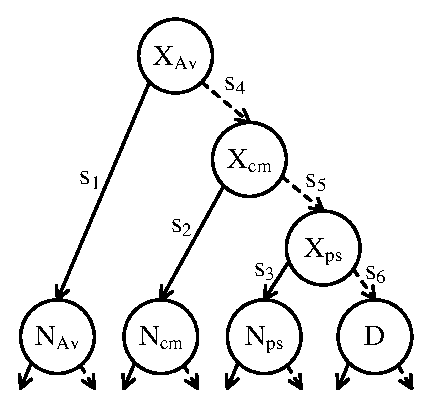
\includegraphics[width=0.35\textwidth]{chap4/CMPSGPDD.eps}
	\bicaption[fig:cmpsgpdd]{多端口方法构造CMRR及PSRR的GPDD结构}{多端口方法构造CMRR及PSRR的GPDD结构}{Fig}{GPDD Structure for multi-port construction of CMRR and PSRR}
\end{figure}

这里的子GPDD结构由$N_{Av}$,$N_{cm}$,$N_{ps}$和$D$这四个GPDD节点为根组成。
我们将使用他们的符号化结果来计算得到CMRR和PSRR的值。
那么根据GPDD的求值规则,辅以符号化电路元件约减的性质,可以得到之前的三个增益可用下式计算得到。

\begin{eqnarray}
A_v     &= \frac{1}{X_{Av}} &= - s_1 s_4 s_5 s_6 \frac{f\left(N_{Av}\right)}{f\left(D\right)}\\
A_{cm}  &= \frac{1}{X_{cm}} &= - s_2 s_5 s_6 \frac{f\left(N_{cm}\right)}{f\left(D\right)}\\
A_{ps}  &= \frac{1}{X_{ps}} &= - s_3 s_6 \frac{f\left(N_{ps}\right)}{f\left(D\right)}
\end{eqnarray}

同时,根据CMRR和PSRR的定义,可以简化CMRR和PSRR在GPDD中的计算如下:

\begin{eqnarray}
CMRR &=& s_1 s_2 s_4 \frac{f\left(N_{Av}\right)}{f\left(N_{cm}\right)}\\
PSRR &=& s_1 s_3 s_4 s_5 \frac{f\left(N_{Av}\right)}{f\left(N_{ps}\right)}
\end{eqnarray}

值得注意的是,这里GPDD的构造过程只需要一次。
只要知道所有电路符号元件的值,而后$A_v$,$CMRR$和$PSRR$的数值结果可以通过自底向上遍历GPDD结构同时得到,节省了计算时间。
这样的计算效率在之前提出的一些符号化方法中是不可行的\parencite{Gielen-ISAAC-1989}。

根据第\ref{chap:gpddtheory}章中介绍的敏感度计算方法,通过简单的推导即可知道,CMRR和PSRR的敏感度也可以通过如下的计算得到:

\begin{equation}
Sens\left( {{CMRR},{W_i}} \right) = Sens\left( {{A_{v}},{W_i}} \right) - Sens\left( {{A_{cm}},{W_i}} \right)
\end{equation}

\begin{equation}
Sens\left( {{PSRR},{W_i}} \right) = Sens\left( {{A_{v}},{W_i}} \right) - Sens\left( {{A_{ps}},{W_i}} \right)
\end{equation}

这意味着我们需要求得三个增益的敏感度,即可得到CMRR和PSRR的敏感度。
同时,由于所有的计算均在同一个GPDD上进行,所以可以高效地求得相应的结果。

\subsection{共模抑制比与电源抑制比测试结果}

\subsubsection{多端口构造方法的双图决策图的时间空间复杂度比较}

这里的测试电路选用了图\ref{fig:two_stage}和图\ref{fig:folded_cascode}中的折叠共源共栅运放和两级运放结构。

\begin{figure}[!htp]
	\centering
	\includegraphics[width=0.7\textwidth]{chap4/res/TSRes.eps}
	\bicaption[fig:trres]{两级运放的$CMRR$及$PSRR$的频率响应结果}{两级运放的$CMRR$及$PSRR$的频率响应结果}{Fig}{Frequency response for $CMRR$ and $PSRR$ in two-stage opamp}
\end{figure}

\begin{figure}[!htp]
	\centering
	\includegraphics[width=0.7\textwidth]{chap4/res/FDRes.eps}
	\bicaption[fig:fcres]{折叠共源共栅运放的$CMRR$及$PSRR$的频率响应结果}{折叠共源共栅运放的$CMRR$及$PSRR$的频率响应结果}{Fig}{Frequency response for $CMRR$ and $PSRR$ in folded-cascode opamp}
\end{figure}

相应的小信号电路元件参数通过HSPICE的数值仿真结果得到,并构建相应的GPDD结构。
计算得到的CMRR和PSRR的频率响应曲线在图\ref{fig:trres}和图\ref{fig:fcres}中展示。
可以看到仿真结构与HSPICE的数值结果十分吻合,所以GPDD符号化计算的结果是有效的。

\begin{table}[!htp]
	\bicaption[tab:tscmpsgpdd]{两级运放的单独构造与多端口构造的时空性能比较}{两级运放的单独构造与多端口构造的时空性能比较}{Table}{Comparison between separated and multi-port constructions for the two-stage opamp}
	\centering
	\begin{tabular}{*{3}{c}}
		\hline
		       情况         & $|\mbox{GPDD}|$ & 构造时间 ($\mu s$) \\ \hline
		 单独构造$A_v$的GPDD   &      2251       &     522.0      \\
		单独构造$A_{cm}$的GPDD &      2615       &     408.7      \\
		单独构造$A_{ps}$的GPDD &      3933       &     632.0      \\
		       总计         &      8799       &     1562.7     \\ \hline
		    多端口构造GPDD     &      4871       &     730.1      \\ \hline
		      改进程度        &     44.6\%      &      2.1x      \\ \hline
	\end{tabular}
\end{table}

\begin{table}[!htp]
	\bicaption[tab:fccmpsgpdd]{折叠共源共栅运放的单独构造与多端口构造的时空性能比较}{两级运放的单独构造与多端口构造的时空性能比较}{Table}{Comparison between separated and multi-port constructions for the folded-cascode opamp}
	\centering
	\begin{tabular}{*{3}{c}}
		\hline
		       情况         & $|\mbox{GPDD}|$ & 构造时间 ($s$) \\ \hline
		 单独构造$A_v$的GPDD   &      24228      &   155.2    \\
		单独构造$A_{cm}$的GPDD &      25706      &   122.0    \\
		单独构造$A_{ps}$的GPDD &      32918      &   173.6    \\
		       总计         &      82852      &   450.8    \\ \hline
		    多端口构造GPDD     &      35424      &    78.7    \\ \hline
		      改进程度        &     57.2\%      &    5.7x    \\ \hline
	\end{tabular}
\end{table}

我们也统计我们的软件实现性能来证明多端口构造得到的GPDD共享结果的优势。
首先,我们针对三种增益$A_v$,$A_{cm}$和$A_{ps}$分别单独构造GPDD结构,并统计相应的构造时间和GPDD节点个数。
其相应的结果在表\ref{tab:tscmpsgpdd}和表\ref{tab:fccmpsgpdd}中展现。
总计一栏将上述三个增益分别的表现进行了求和,反映分别构造总复杂度。
然后采用多端口方式构造同时对三个增益构造GPDD。
从表中的数据可以明显地看到多端口电路构造方式的优势,利用更少的时间和更少的计算空间完成了整体的计算。

\subsubsection{两级运放的电路的参数扫描结果}

由于符号化一次构造,多次计算的优良性质,符号化计算可以快速地对电路的参数进行扫描,并从中观察电路元件取值对电路性能的影响。
这里我们对两级运放的补偿部分的两个电路元件补偿电容$C_c$和调零电阻$R_z$进行参数扫描,以观察CMRR和PSRR与其之间的关系。

\begin{figure}[!htp]
	\centering
	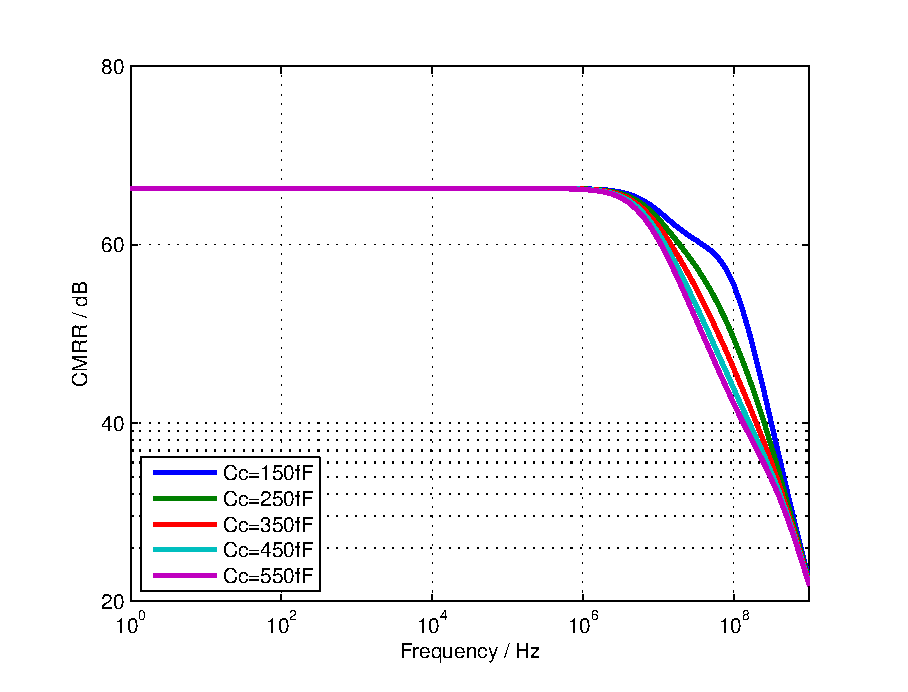
\includegraphics[width=0.7\textwidth]{chap4/res/CMRR_CC.eps}
	\bicaption[fig:cmrrcc]{两级运放针的$CMRR$对补偿电容$C_c$的参数扫描结果}{两级运放针的$CMRR$对补偿电容$C_c$的参数扫描结果}{Fig}{Parameter sweep results for $CMRR$ of compensation capacitor $C_c$ in two-stage opamp}
\end{figure}

\begin{figure}[!htp]
	\centering
	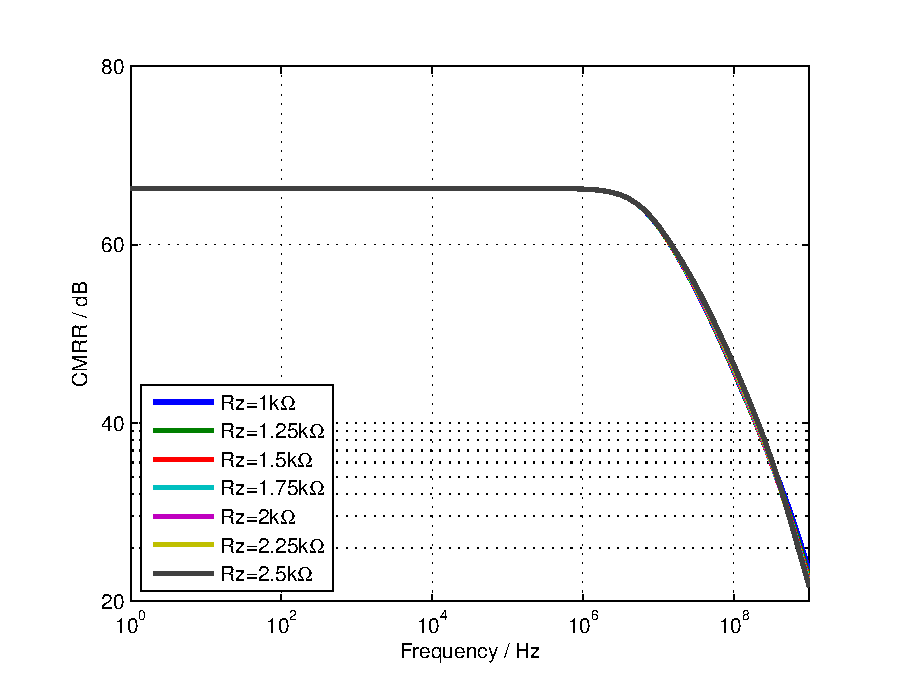
\includegraphics[width=0.7\textwidth]{chap4/res/CMRR_Rz.eps}
	\bicaption[fig:cmrrrz]{两级运放针的$PSRR$对调零电阻$R_z$的参数扫描结果}{两级运放针的$CMRR$对补偿电容$R_z$的参数扫描结果}{Fig}{Parameter sweep results for $CMRR$ of compensation capacitor $R_z$ in two-stage opamp}
\end{figure}

\begin{figure}[!htp]
	\centering
	\includegraphics[width=0.7\textwidth]{chap4/res/PSRR_CC.eps}
	\bicaption[fig:psrrcc]{两级运放针的$PSRR$对补偿电容$C_c$的参数扫描结果}{两级运放针的$PSRR$对补偿电容$C_c$的参数扫描结果}{Fig}{Parameter sweep results for $PSRR$ of compensation capacitor $C_c$ in two-stage opamp}
\end{figure}

\begin{figure}[!htp]
	\centering
	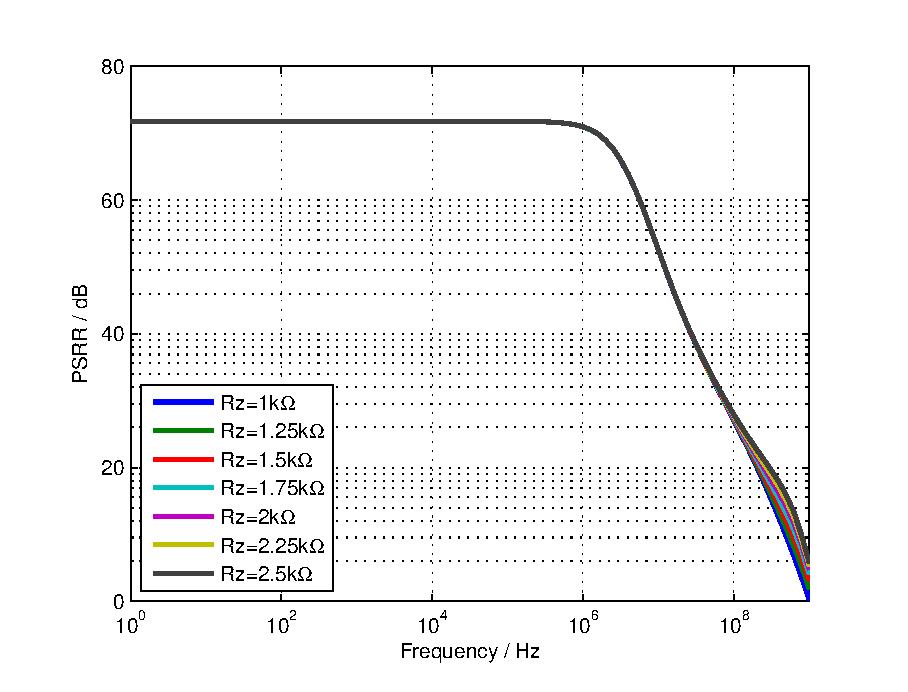
\includegraphics[width=0.7\textwidth]{chap4/res/PSRR_Rz.eps}
	\bicaption[fig:psrrrz]{两级运放针的$PSRR$对调零电阻$R_z$的参数扫描结果}{两级运放针的$PSRR$对补偿电容$R_z$的参数扫描结果}{Fig}{Parameter sweep results for $PSRR$ of compensation capacitor $R_z$ in two-stage opamp}
\end{figure}

根据图\ref{fig:cmrrcc}至图\ref{fig:psrrrz}的结果,可以看到CMRR和PSRR在高频接近转角频率处对于补偿电容$C_c$的变化较为敏感;
然而在同样的区域调零电阻的影响相对小了很多。
根据这些信息,电路工程师可以更方便地观察不同元件取值的影响,从而更有效率地进行电路设计。

\subsubsection{敏感度方法进行电路参数优化共模电源抑制比}

最后,我们对CMRR和PSRR的敏感度进行计算,并尝试通过敏感度进行电路优化。
这里仍然针对两级运放进行分析,我们对其中的第一级和第二级的输入MOS管$M_1$和$M_6$的尺寸求取敏感度。
相应的敏感度结果在图\ref{fig:SensW6}和图\ref{fig:SensW6}中展现。

\begin{figure}[!htp]
	\centering
	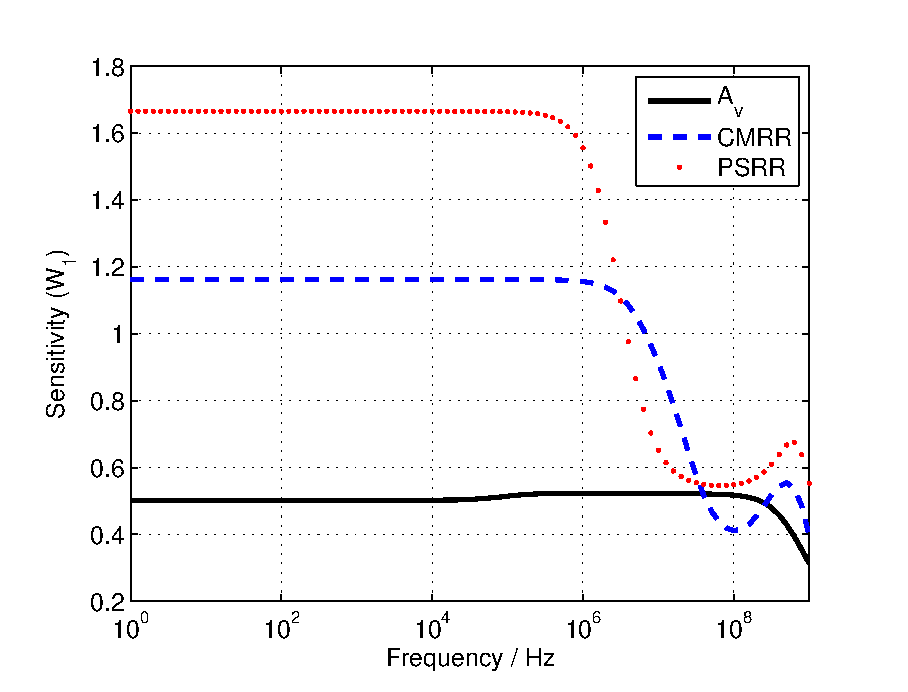
\includegraphics[width=0.7\textwidth]{chap4/res/SensW1.eps}
	\bicaption[fig:SensW1]{两级运放针对$W_1$的敏感度分析结果}{两级运放针对$W_1$的敏感度分析结果}{Fig}{Sensitivity results of $W_1$ in two-stage opamp}
\end{figure}

\begin{figure}[!htp]
	\centering
	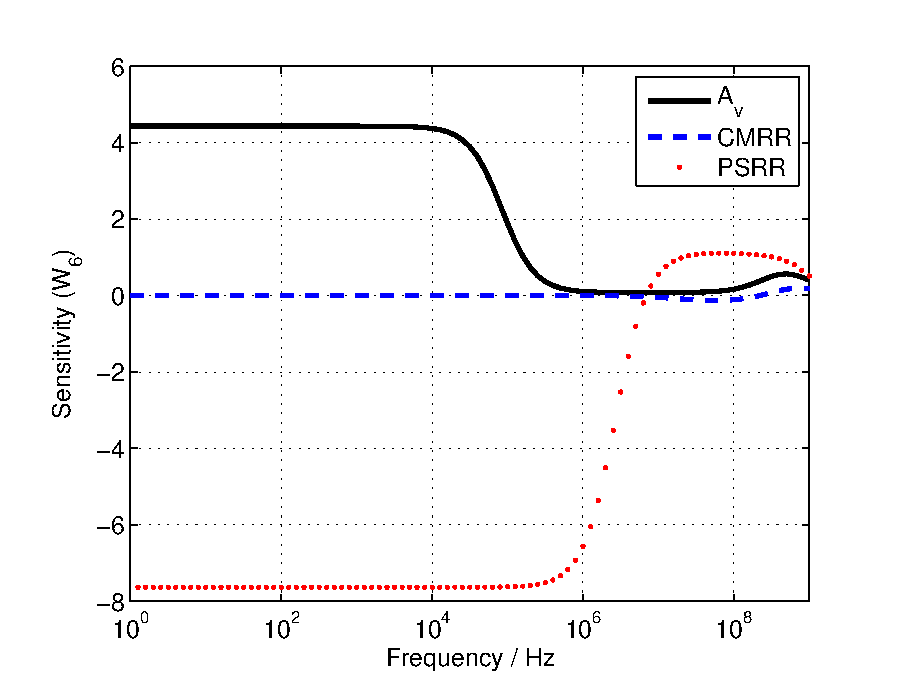
\includegraphics[width=0.7\textwidth]{chap4/res/SensW6.eps}
	\bicaption[fig:SensW6]{两级运放针对$W_6$的敏感度分析结果}{两级运放针对$W_6$的敏感度分析结果}{Fig}{Sensitivity results of $W_6$ in two-stage opamp}
\end{figure}

根据图中所展现的结果,我们看到$W_1$与三种电路指标$A_v$、$CMRR$和$PSRR$均正相关,故增大$W_1$将同时增大三种性能指标。
然而$W_6$情况则不同,如增大$W_6$的话,差分增益$A_v$会有所提升,$CMRR$基本保持不变,而$PSRR$则会下降。

我们在实际对运放进行了尺寸优化($W_1$从原有的$20\mu m$变为$30\mu m$,$W_6$从原有的$30\mu m$变为$31\mu m$)后,将相应的数据变化记录于表\ref{tab:sensw1}和表\ref{tab:sensw6}中。

\begin{table}[!htp]
	\bicaption[tab:sensw1]{$W_1$的DC敏感度分析结果及优化}{$W_1$的DC敏感度分析结果及优化}{Table}{Sensitivity analysis at DC of $W_1$}
	\centering
	\begin{tabular}{c|c|c|c|c|c}
		\hline
		\multirow{2}{*}{指标} & \multicolumn{2}{c|}{$W_1=20\mu m$} & \multicolumn{2}{c|}{$W_1=30\mu m$} & \multirow{2}{*}{比率} \\ \cline{2-5}
		                    &       值        &        敏感度        &       值        &        敏感度        &  \\ \hline
		       $A_v$        & 2.84K (69.1dB) &       0.502       & 3.41K (70.7dB) &       0.401       &  +20.0\% (+1.6dB)   \\ \hline
		      $CMRR$        & 2.07K (66.3dB) &       1.162       & 3.05K (69.7dB) &       0.802       &  +47.3\% (+3.4dB)   \\ \hline
		      $PSRR$        & 3.87K (71.8dB) &       1.665       & 6.92K (76.8dB) &       1.237       &  +78.8\% (+5.0dB)   \\ \hline
	\end{tabular}
\end{table}

\begin{table}[!htp]
	\bicaption[tab:sensw6]{$W_6$的DC敏感度分析结果及优化}{$W_6$的DC敏感度分析结果及优化}{Table}{Sensitivity analysis at DC of $W_6$}
	\centering
	\begin{tabular}{c|c|c|c|c|c}
		\hline
		\multirow{2}{*}{指标} & \multicolumn{2}{c|}{$W_6=30\mu m$} & \multicolumn{2}{c|}{$W_6=31\mu m$} & \multirow{2}{*}{比率} \\ \cline{2-5}
		                    &       值        &        敏感度        &       值        &        敏感度        &  \\ \hline
		       $A_v$        & 2.84K (69.1dB) &       4.43        & 3.04K (69.7dB) &       -0.20       &  +7.04\% (+0.6dB)   \\ \hline
		      $CMRR$        & 2.07K (66.3dB) &      6.1e-8       & 2.07K (66.3dB) &      9.4e-8       &     +0\% (+0dB)     \\ \hline
		      $PSRR$        & 3.87K (71.8dB) &       -7.63       & 3.32K (70.4dB) &       -2.83       &  -14.2\% (-1.4dB)   \\ \hline
	\end{tabular}
\end{table}

可以看到在尺寸调整后,三种电路指标$A_v$、$CMRR$和$PSRR$均按预期发生了变化。
同时由于敏感度的定义,即可知道电路性能变化比率与敏感度基本成正比,这在表中的数据也得到了相应的验证。
高敏感度带来了更快的性能增长。
另外,还应观察到在电路尺寸改变后电路的敏感度也发生了变化。
例如,表\ref{tab:sensw6}中的有关$A_v$的敏感度已经由正值变为了负值,说明继续增大$W_6$将对电路的增益带来不好的效果。

\section{本章小结}

本章介绍了本论文中所用到电路简化原理的两种应用,分别为时域模型建立和CMRR、PSRR分析。

师傅分析部分主要回顾了时域模型生成方法的相关历史,并提出了自己的时域模型简化方法,并对方法进行了测试。
这种方法的优势在于其生成的模型是符号化的,并且大部分流程可以自动化,不需要过多的电路经验也可以对电路模型进行分析。
可以看到目前符号化时域简化模型分析方法仅针对部分电路可以成功使用,但是仍有许多电路存在分析困难的情况。
需要进一步通过非线性函数选取和系统层面理论分析对电路模型生成的方法进行论证。

CMRR和PSRR分析中将多端口符号化构造方法用于其分析当中,介绍$CMRR$和$PSRR$的计算流程,并利用敏感度分析方法有电路进行调整优化。
最后,通过GPDD构造的高效性,用参数扫描分析以及敏感性分析辅助电路优化等测试证明了这种构造方法的有效性。